%
% db-poissonverteilung.tex -- Datenblatt der Poisson-Verteilung
%
% (c) 2015 Prof Dr Andreas Mueller, Hochschule Rapperswil
%
\subsection{Steckbrief}
\begin{center}
\renewcommand{\arraystretch}{1.5}
\begin{tabular}{|l|l|}
\hline
Name&Poissonverteilung\\
\hline
Wahrscheinlichkeit&
\begin{minipage}{3.7in}
\vskip3pt
$\displaystyle
P_\lambda(k)=\frac{\lambda^k}{k!}e^{-\lambda}
$
\end{minipage}
\\
Erwartungswert&$\displaystyle \lambda$\\
Varianz&$\displaystyle \lambda$\\
\hline
Anwendungen&\begin{minipage}{3.7in}%
\vskip3pt
\strut
$\bullet$ Anzahl Ereignisse mit exponentialverteilten Intervallen\\
$\bullet$ Approximation der Binomialverteilung f"ur seltene Ereignisse, die
mit Rate $\lambda$ eintreten
\strut
\end{minipage}\\[20pt]
\hline
\end{tabular}
\end{center}

\subsection{Wahrscheinlichkeitsverteilung}
Wahrscheinlichkeitsverteilung der Poisson-Verteilung f"ur
$\lambda=4.2$, $E(X)=\lambda$ und $\operatorname{var}(X)=\sqrt{\lambda}$.
\begin{center}
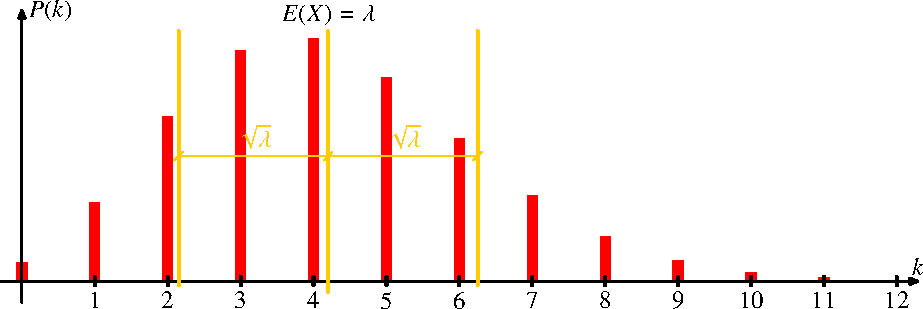
\includegraphics{images/exp-2.pdf}
\end{center}

\subsection{Sch"atzung des Parameters \texorpdfstring{$\lambda$}{lamda}}
Der Parameter $\lambda$ ist der Erwartungswert einer Poisson-Verteilung,
er l"asst sich daher mit dem Mittelwert
\[
\hat\lambda(k_1,\dots,k_n)=\frac{k_1+\dots+k_n}n
\]
erwartungstreu sch"atzen.

